{
% Image scale
\def\imgscale{0.34}

\textsf{Vi vil i det følgende forklare vores tanker bag en meget simpelt
fremgangsmåde som skal afgøre om et billede fremviser brug af det gyldne
snit. For at afgøre dette, trækker vi sammenhængende regioner ud af
billedet og vurderer dem efter deres placering, størrelse og form. I
denne sammenhæng bør en regions \emph{kant} forstås som en side af det
rektangel, der afgrænser en given region.}

\subsubsection{Regionens placering}
Den naive løsning går ud på at lave et meget simpelt check om hvorvidt
et billede opfylder det gyldne snit. Vi siger at et billede
opfylder det gyldne snit, hvis en interessant region tangerer den linje
der deler et billede efter det gyldne snit. Et eksempel er vist i figur
\ref{pos_naiv_1}, hvor regionen vi betragter er farvet sort. Den røde
linje markerer det gyldne snit. Dette farvskema vil være gennemgående i
det følgende.
\begin{figure}[h]
	\begin{center}
		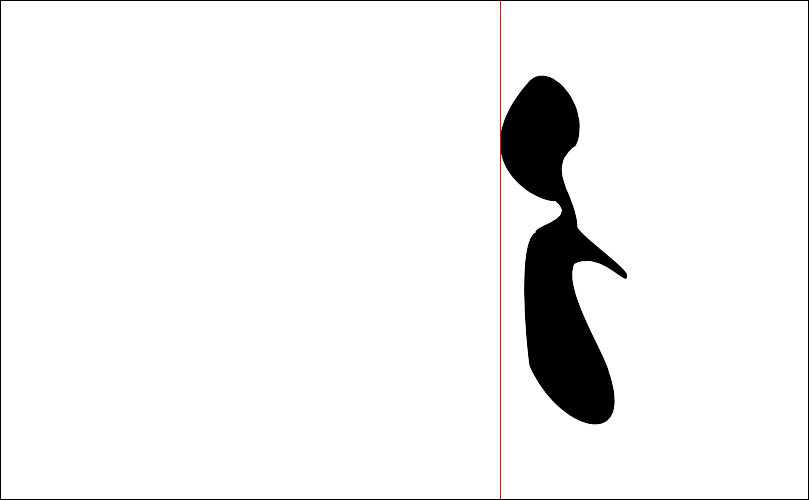
\includegraphics[scale=\imgscale,angle=0]{afsnit/vores_implementation/billeder/naiv_algoritme/naiv_positiv_blob_1}
	\end{center}
	\caption[En positiv region]{En sammenhængende region som tangerer det gyldne snit.
	Denne region er positiv.}
	\label{pos_naiv_1}
\end{figure}

I figur \ref{pos_naiv_1} er vi dog heldige, idet regionen virkelig
\emph{kan} klassificeres som interessant fordi billedet er meget simpelt. I
praksis vil vi have mange regioner, hvor vi gerne vil fjerne de regioner
der ikke kan klassificeres som interessante. Figur
\ref{realworld_example} viser hvordan et rigtigt maleri kunne se ud, når
vi gerne vil bestemme interessante regioner.
\begin{figure}[p]
	\begin{center}
		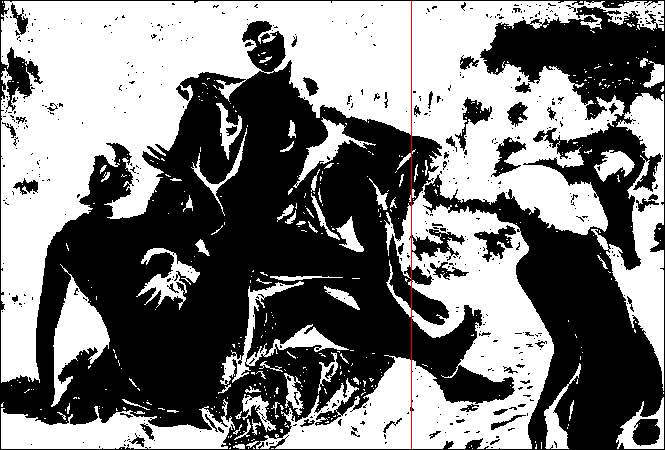
\includegraphics[scale=0.42,angle=0]{afsnit/vores_implementation/billeder/naiv_algoritme/bathers_mockup_blob}
	\end{center}
	\caption[Interessante regioner i praksis]{I praksis vil de
	fundne regioner være langt mere komplekse.}
	\label{realworld_example}
\end{figure}

Billedet i figur \ref{realworld_example} viser nogle komplekse regioner,
men ingen er interessante set i forhold til vores meget simple
definition, da ingen af disse regioner tangerer snittet som vist i figur
\ref{pos_naiv_1}.  Generelt kan vi sige, at hvis en region krydser
snittet kan denne ikke siges at ligge i det gyldne snit. En simpel
illustration på dette vises i figur \ref{neg_naiv_1}.
\begin{figure}[p]
	\begin{center}
		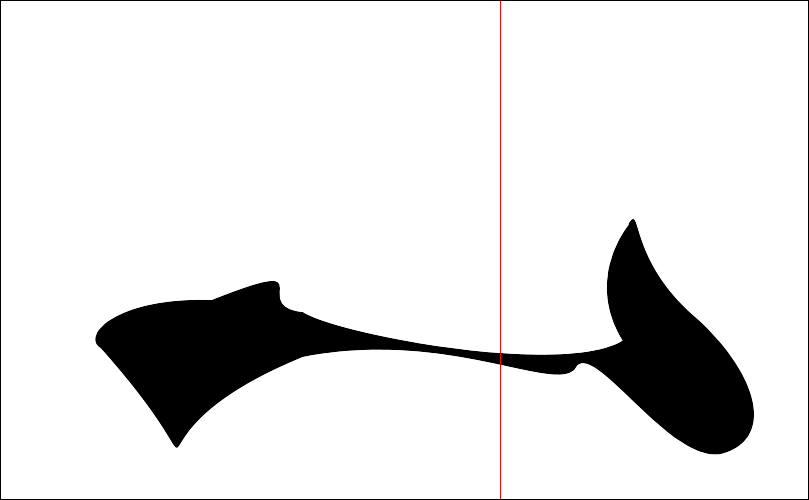
\includegraphics[scale=\imgscale,angle=0]{afsnit/vores_implementation/billeder/naiv_algoritme/naiv_negativ_blob_2}
	\end{center}
	\caption[En negativt region]{En sammenhængende region som krydser snittet kan ikke
	betragtes som at den opfylder det gyldne snit. Denne region en
	negativ.}
	\label{neg_naiv_1}
\end{figure}

Da vi ikke kan regne os helt nøjagtigt frem til $\varPhi$ når vi
kun har heltal at arbejde med, indfører vi nu en margen hvor vil vil
acceptere regioner. I praksis betyder dette at vi ikke \emph{kun} kigger
på den linje der deler billedet ved det gyldne snit, men også ved siden
af den. Derved behøver en region ikke at tangere det gyldne snit helt
nøjagtig for at kunne betragtes som en interessant region. F.eks. vil
regionen i figur \ref{pos_naiv_margin_1} anses som værende placeret i
det gyldne snit. Vær opmærksom på at vores margen, rent visuelt i de
følgende illustrationer, er stærkt overdrevet.
\begin{figure}[h]
	\begin{center}
		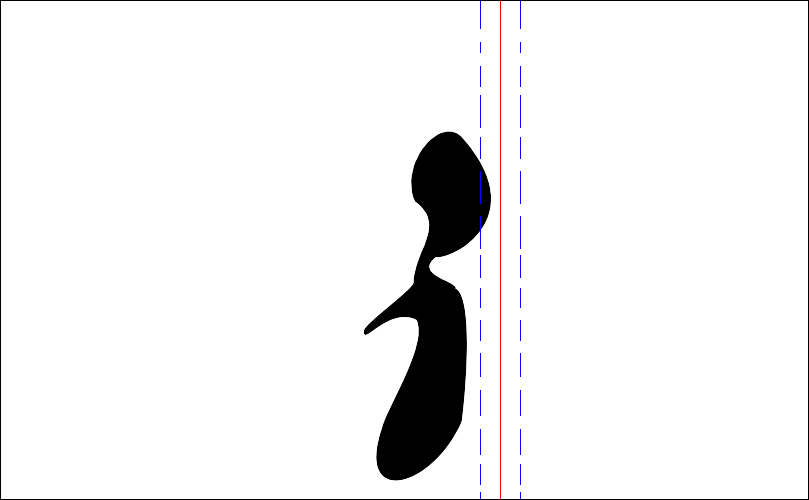
\includegraphics[scale=\imgscale,angle=0]{afsnit/vores_implementation/billeder/naiv_algoritme/naiv_positiv_blob_margin_1}
	\end{center}
	\caption[Positiv region i margen]{En sammenhængende region som ligger indenfor en margen
	af det gyldne snit betragtes som positiv.}
	\label{pos_naiv_margin_1}
\end{figure}

\subsubsection{Regionens størrelse}
Med vores nuværende definition på hvornår en region kan betegnes som
interessant, skal vi blot have en sammenhængende region indenfor en
margen af det gyldne snit. Hvis vi kaster et blik tilbage på figur
\ref{realworld_example} ses det at der i dette tilfælde vil blive
udvalgt mange små regioner som egentlig ikke kan tillægges nogen
betydning. Vi siger derfor at en sammenhængende region skal have en vis
størrelse før den kan tages i betragtning. I praksis vil regionens areal
afspejle dens størrelse, hvor arealet er det antal pixels regionen
optager i billedet. Grænsen for et acceptabelt areal skal sættes i
forhold til billedets størrelse.

Omvendt er vi heller ikke interesseret i at få for store regioner med i
betragtningerne. F.eks. vil en himmel i et maleri give en ret stor
sammehængende region. De fleste af sådanne regioner vil dog ikke blive
taget i betragtning fordi de krydser snittet. Hvis vi kigger på det
meget simple billede i figur \ref{pos_naiv_1} skal man også huske på at
der faktisk vises to regioner. Den sorte skikkelse er en sammenhængende
region ligesom den hvide baggrund er en sammenhængende region.
Baggrunden kan ikke siges at være en interessant region, hvorfor det er
vigtigt at sortere disse regioner fra.

Indtil videre har vi kun illustreret ét snit i billedet. Der er
imidlertid tre andre snit hvor vi også kan dele et billede efter det
gyldne snit. Hvor vi nu har kigget på et vertikalt snit, vender vi nu
opmærksomheden mod et horisontalt snit. Det generelle tilfælde vil
være\footnote{Total påstand} at en region kun er interessant i forhold
til enten et vertikalt eller et horisontalt snit. Et eksempel på dette
ses i figur \ref{pos_horiz_naiv_margin_1}.
\begin{figure}[H]
	\begin{center}
		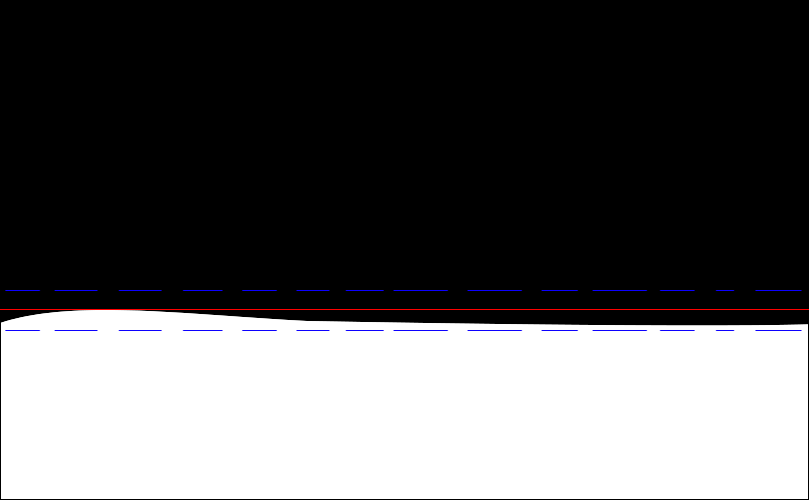
\includegraphics[scale=\imgscale,angle=0]{afsnit/vores_implementation/billeder/naiv_algoritme/naiv_horiz_positiv_blob_1}
	\end{center}
	\caption[Positiv horisontal region]{En positiv sammenhængende region som findes indenfor
	margen uden at krydse snittet.}
	\label{pos_horiz_naiv_margin_1}
\end{figure}
Det ses tydeligt at regionen i figur \ref{pos_horiz_naiv_margin_1} ikke
kan tages i betragtning i forhold til et vertikalt snit, da regionen,
uanset snittets placering, vil krydse dette. Det ses dog at regionen
holder sig indenfor margen i forhold til et horisontalt snit og derfor
kan klassificeres som en interessant region der opfylder det gyldne
snit.

\subsubsection{Regionens form}
Regionens form kan også give informationer om hvorvidt vi har med en
interessant region at gøre. I praksis er det dog meget svært at sige
noget om selve den fysiske form af en region, men vi kan sige noget om
dens masse. En regions masse skal forstås som forholdet mellem regionens areal og
arealet af det rektangel der afgrænser regionen. Dette forhold giver
information om ``hvor massiv'' en region er. En massiv region vil være
mere interessant end en meget spinkel region. Figur \ref{region_mass}
illustrerer to forskellige regioner med forskellig masse.
\begin{figure}[h]
	\begin{center}
		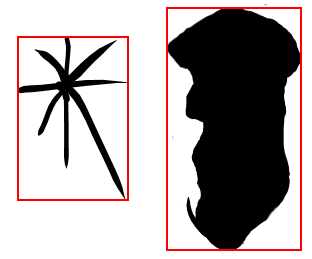
\includegraphics[scale=\imgscale,angle=0]{afsnit/vores_implementation/billeder/naiv_algoritme/bbox_area_ratio}
	\end{center}
	\caption[Regioners masse]{To forskellige regioner med vidt forskellige forhold
	mellem selve regionens areal og arealet af det rektangel der
	afgrænser regionen.}
	\label{region_mass}
\end{figure}

\subsubsection{Sammenfatning}
Vi samler nu op på de ovenstående krav for bestemmelse af en interessant
region liggende i det gyldne snit.

For at en region kan betegnes som liggende i det gyldne snit skal den
\begin{enumerate}
	\renewcommand{\labelenumi}{(\alph{enumi})}
	\item tangere den linje der deler billedet efter det gyldne snit
	\item eller have en kant indenfor en margin af det gyldne snit
\end{enumerate}
og regionen må \textbf{ikke}
\begin{enumerate}
	\renewcommand{\labelenumi}{(\alph{enumi})}
	\setcounter{enumi}{2}
	\item krydse linjen der deler billedet efter det gyldne snit;
	\item have en bounding box der ligger udenfor margen;
	\item have et areal mindre end en variabel tærskel der sættes i
		forhold til billedets størrelse
	\item eller have en masse mindre end variabel tærskel.
\end{enumerate}
Vi har da at en region skal opfylde
\begin{equation}
	(a \vee b) \wedge \neg (c \vee d \vee e \vee f)
\end{equation}
før at den kan betegnes som liggende i det gyldne snit. Vi vil senere
komme ind på hvordan vi for en given region afgør om den opfylder
ovenstående betingelser.

}

% vim: set tw=72 spell spelllang=da:
